\documentclass[9pt,a4paper,titlepage,oneside,mathserif,serif]{beamer}
\usepackage[latin1]{inputenc}
\usepackage{amsmath}
\usepackage{amsfonts}
\usepackage{amssymb}
\usepackage{graphicx}
\usepackage{algorithm2e} 

\usepackage[procnames]{listings}
\usepackage{color}

\author{Leonhard Applis}
\title{Classifier Explanation}
\subtitle{Introduction to the Algorithms LIME and SP-LIME}
\institute{TH N�rnberg} % (optional)
\date{21.1.2019}
\subject{BigDataSystems}

\usetheme{PaloAlto}
%% \usecolortheme{beaver}
\AtBeginSection[]
{
\begin{frame}
	\frametitle{Table of Contents}
	\tableofcontents[currentsection,currentsubsection]
\end{frame}
}
%%------------------ for longer presentations required
\pgfmathsetmacro{\progress}{\insertframestartpage/\inserttotalframenumber}
%%------------------ To Show PythonCode with Lstlistings
\definecolor{keywords}{RGB}{255,0,90}
\definecolor{comments}{RGB}{0,0,113}
\definecolor{red}{RGB}{160,0,0}
\definecolor{green}{RGB}{0,150,0}
\definecolor{black}{RGB}{0,0,0}

\lstset{language=Python, 
	basicstyle=\ttfamily\small, 
	keywordstyle=\color{keywords},
	commentstyle=\color{green},
	stringstyle=\color{comments},
	showstringspaces=false,
	identifierstyle=\color{black},
	procnamekeys={def,class}}


\begin{document}
\frame{\titlepage}
\frame{\tableofcontents}
\section{Basics}
\begin{frame}
	\frametitle{Trusting a Prediction}
	What do Humans need to unterstand a Prediction
\end{frame}
\begin{frame}
	\frametitle{Example}
	Maybe just pick the Atheist Christian Example from the paper
\end{frame}
\begin{frame}
	\frametitle{Trusting a Model}
	Whats the next step after trusting a single prediction
	
	Mention time-required for manually checking a lot of pictures
\end{frame}
\begin{frame}
	\frametitle{Example}
	
\end{frame}
\begin{frame}
	\frametitle{Prooving a Model}
	Classifier Explanation is required to set anything up IRL, or everyone will hate you very bad
\end{frame}
\begin{frame}
	\frametitle{Improving a Model}
	How Classifier Explanation helps you to improve your models
	
	Better Filtering
	Maybe better weighting of features
	Finding Links in Classification (Similiar Classes?)
\end{frame}
\section{LIME}
\begin{frame}
	\frametitle{Requirements}
	\begin{Large}
		\textbf{What do we want:}
		\begin{itemize}
			\item Human Readable Model Explanation
			\item For Every Classifier
			\item For Every Input
		\end{itemize}
	~\newline
	\begin{center}
		\textbf{ features $\neq$ human readable }
	\end{center}
	~\newline
	\end{Large}
	To gain $readability$: 
	\begin{itemize}
		\item show influence relative to each other, not as numbers
		\item only show most important features
		\item use \textit{superpixels} instead of pixels
	\end{itemize}
\end{frame}

\begin{frame}
	\frametitle{Definitions}
	Let:
	\begin{enumerate}
		\item $G$ be any possible explanation model
		\item $g$ be our explanation Model
		\item $\Omega(g)$ the complexity of our Model
		\begin{itemize}
			\item Weights in a regressions model
			\item Depth of an decisiontree
			\item Number of trees in a random forest
		\end{itemize}
		\item $f: Features -> Class $ be the real classification
		\item $\Pi_x(z)$ as proximity-measure from $x$ to $z$
		\item $\mathcal{L}(f,g,\Pi_x)$ measure of un-faithfullness of $g$ compared to $f$ given the proxmity $\Pi_x$
	\end{enumerate}
\end{frame}

\begin{frame}
	\frametitle{Minimizing Fidelity $\cdot$ Interpretability}
	\begin{Large}
		Wanted: ~\newline
		\begin{center}
			$\xi(x) = argmin_{g\in G} ~ \mathcal{L}(f,g,\Pi_x) + \Omega(g)$
		\end{center}
		Read: 
		\begin{itemize}
			\item We want for every input $x$
			\item an explanation(-model)
			\item where complexity of $g$ and the failure of $g$ are minimal
			\item given a set of possible explanations $G$
		\end{itemize}
	\end{Large}
~\newline ~\newline 
We do so by picking samples $x^,$ as subsets from an input $x$ and \textbf{optimizing} our model $g$ \footnote{We do not really check different models, we train one} 
\end{frame}

\begin{frame}
	\frametitle{Local Interpretable Model-Agnostic Explanations}
	\framesubtitle{The LIME-Algorithm}
	Additional Requirements: ~\newline 
	\textbf{LASSO}\footnote{Further Reading: \url{https://beta.vu.nl/nl/Images/werkstuk-fonti_tcm235-836234.pdf}} - \textit{Least Absolute Shrinkage and Selection Operator} ~\newline 
	Machine Learning algorithm to select most important features relative to each other. ~\newline
	G are only \textit{sparse linear regression models} (e.g. Decision Trees or simple logistic regression) ~\newline 
	
%	\begin{algorithm}[H]
%		\SetKwInOut{Require}{Require}
%		\Require{Classifier $f$, Number of samples $N$}
%		\Require{Instance $x$, and its interpretable version $x^,$}
%		\Require{Similarity kernel $\pi_x$, Length of explanation $K$}
%		$\mathcal{Z} \leftarrow \{\}$\;
%		\ForEach{$i \in \{1,2,..,N\}$}{
%		$z^,_i \leftarrow sample\_around(x^,)$\;
%		$\mathcal{Z} \leftarrow \mathcal{Z} \cup \<z^,_i ,f(z_i,\pi_x(z_i)) \>$\;
%		}
%		$ w \leftarrow K-Lasso(\mathcal{Z},K)  \triangleright~ with~ z^,_i~ as~ features,~ f(z) ~ as ~ target$\;
%		return  $w$\;
%	\end{algorithm}

\end{frame}
\section{Example: Traffic Sign Recognition}

\begin{frame}
	\frametitle{Trafficsign-Recognition}
	\framesubtitle{Explaining a neural network}
	\begin{Large}
		given neural network :
		\begin{itemize}
				\item 6 layers, first 3 convolutional (complex structure)
				\item 43 Classes (complex output)
				\item 64x64 Images (complex input) 
				\item trained with 8k images (rich data-input)
				\item tested with 2k images reaching 95\% accuracy (good?)
		\end{itemize}
	\end{Large}
	The NN was trained with Tensorflow and is shipped with your notebook. 
\end{frame}

\begin{frame}
	\frametitle{Trafficsign-Recognition}
	\framesubtitle{How to}
	\lstinputlisting{TexFiles/LimeSnippet.py}
\end{frame}

\begin{frame}
	\frametitle{Trafficsign-Recognition}
	\framesubtitle{Simple Classification}
	
	\begin{columns}
		\begin{column}{0.33\textwidth}
			\begin{center}
				\begin{figure}[H]
					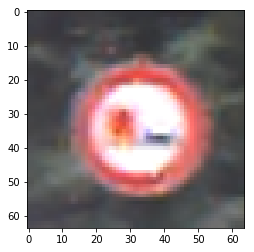
\includegraphics[width=0.9\linewidth]{Images/NoOvertaking}
					\caption[No Overtaking]{No Overtaking - Sample Image from Test-data}
					\label{fig:noovertaking}
				\end{figure}
			\end{center}		
		\end{column}
		\begin{column}{0.33\textwidth}
			\begin{center}
				\begin{figure}[H]
					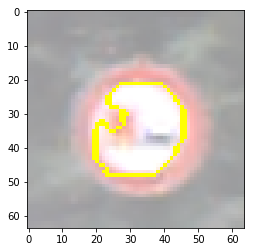
\includegraphics[width=0.9\linewidth]{Images/NoOvertakingCorrectClass}
					\caption[Prediction:  No Overtaking]{ Prediction - showing the 5 Superpixels for \textit{no overtaking}}
					\label{fig:noovertakingCorrect}
				\end{figure}
			\end{center}
		\end{column}
		\begin{column}{0.33\textwidth}
		\begin{center}
			\begin{figure}[H]
				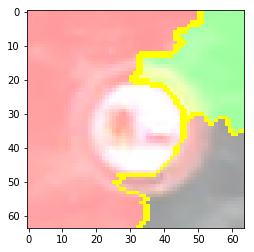
\includegraphics[width=0.9\linewidth]{Images/NoOvertakingFalseClass}
				\caption[Prediction:  right of way crossing]{ Prediction - showing the 4 most important Superpixels for \textit{right of way crossing}}
				\label{fig:noovertakingFalse}
			\end{figure}
		\end{center}
		\end{column}
	\end{columns}
\end{frame}

\begin{frame}
	\frametitle{Trafficsign-Recognition}
	\framesubtitle{Overfitting}
	\begin{columns}
		\begin{column}{0.33\textwidth}
			\begin{center}
				\begin{figure}
					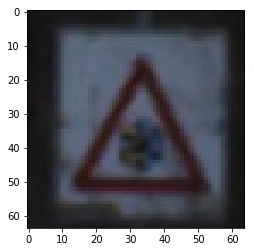
\includegraphics[width=0.9\linewidth]{Images/Frost}
					\caption[Frost]{Frost - Sample Image from \textit{Training}-data}
					\label{fig:frost}
				\end{figure}
			\end{center}		
		\end{column}
		\begin{column}{0.33\textwidth}
			\begin{center}
				\begin{figure}
					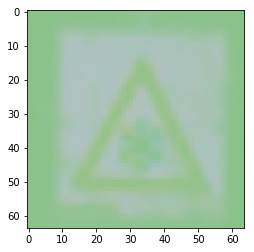
\includegraphics[width=0.9\linewidth]{Images/FrostOverfitting}
					\caption[Prediction:  Frost]{ Prediction for \textit{Frost}, a sign for overfitting}
					\label{fig:frostOverfit}
				\end{figure}
			\end{center}
		\end{column}
	\end{columns}
\end{frame}

\begin{frame}
	\frametitle{Trafficsign-Recognition}
	\framesubtitle{Similiar Classes I}
	\begin{columns}
		\begin{column}{0.33\textwidth}
			\begin{center}
				\begin{figure}
					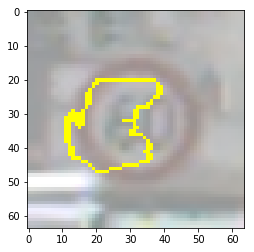
\includegraphics[width=0.9\linewidth]{Images/60Prediction}
					\caption[60]{Prediction: 60 - only 6 is circled}
					\label{fig:60Pred}
				\end{figure}
			\end{center}		
		\end{column}
		\begin{column}{0.33\textwidth}
			\begin{center}
				\begin{figure}
					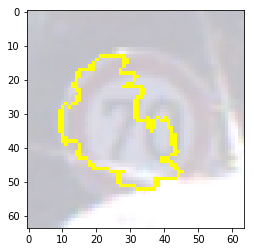
\includegraphics[width=0.9\linewidth]{Images/70Prediction}
					\caption[70]{Prediction: 70 - only 7 is circled}
					\label{fig:70Pred}
				\end{figure}
			\end{center}
		\end{column}
	\end{columns}
	\begin{center}	
		\textbf{The model seems to recognize numbers!}
	\end{center}
\end{frame}

\begin{frame}
\frametitle{Trafficsign-Recognition}
\framesubtitle{Similiar Classes II}
\begin{center}	
	Let's have some fun!
\end{center}
\begin{columns}
	\begin{column}{0.33\textwidth}
		\begin{center}
			\begin{figure}
				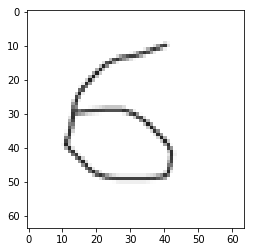
\includegraphics[width=0.9\linewidth]{Images/6Image}
				\caption[6]{Only number 6, no Street Sign}
				\label{fig:6}
			\end{figure}
		\end{center}		
	\end{column}
	\begin{column}{0.33\textwidth}
		\begin{center}
			\begin{figure}
				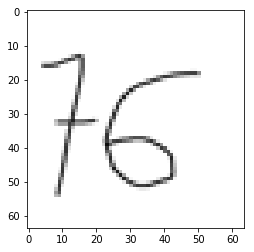
\includegraphics[width=0.9\linewidth]{Images/76Image}
				\caption[76]{Number 76 - what will be predicted?}
				\label{fig:76}
			\end{figure}
		\end{center}
	\end{column}
\end{columns}
\end{frame}

\begin{frame}
\frametitle{Trafficsign-Recognition}
\framesubtitle{Similiar Classes III}
\begin{center}	
	Let's have some fun!
\end{center}
\begin{columns}
	\begin{column}{0.33\textwidth}
		\begin{center}
			\begin{figure}
				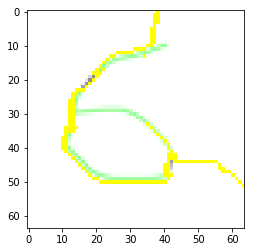
\includegraphics[width=0.9\linewidth]{Images/6Prediction}
				\caption[6]{Number  6  - ~~~ 78\% \textit{Speed Limit 60}}
				\label{fig:6Pred}
			\end{figure}
		\end{center}		
	\end{column}
	\begin{column}{0.33\textwidth}
		\begin{center}
			\begin{figure}
				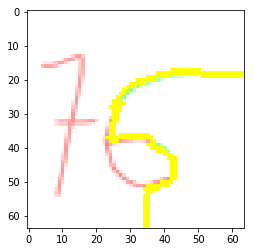
\includegraphics[width=0.9\linewidth]{Images/76Prediction}
				\caption[76]{Number 76 - 99.9\% \textit{No Overtaking}}
				\label{fig:76Pred}
			\end{figure}
		\end{center}
	\end{column}
\end{columns}
\end{frame}

\begin{frame}
	\frametitle{Trafficsign-Recognition}
	\framesubtitle{Conclusion}
	\begin{LARGE}
		\begin{itemize}
			\item Accuracy $\neq$ Quality
			\item most of the predictions \textit{look good}
			\item trainings-data is heavily overfitted
			\item everything that is not a streetsign causes trouble
			\item there can (still) be much more \textit{hidden} problems
		\end{itemize}
	\end{LARGE}
\end{frame}
\begin{frame}
	\frametitle{Thanks}
	\begin{Huge}
		\begin{center}
			Questions?
		\end{center}
	\end{Huge}
\end{frame}

\begin{frame}
	\frametitle{Referendums-Questions}
	\begin{LARGE}
		\begin{itemize}
			\item give an example of unreadable features and it's human-readable LIME-Interpretation
			\item name some measures to improve your model after using the explanations
			\item what is the main difference between LIME and ANCHOR
		\end{itemize}
	\end{LARGE}
\end{frame}
%\section{SP-LIME}

\begin{frame}
	\frametitle{Problem with Sampling}
	Explain that we have to little time to inspect everything
	Looking for a new way to pick samples
\end{frame}

\begin{frame}
	\frametitle{Submodular Pick}
	\framesubtitle{The SPLIME Algorithm}
	Here is the Pseudocode
\end{frame}

\begin{frame}
	\frametitle{SPLIME Example}
	I guess this needs more than 2 Pages, we should add an example 
\end{frame}
\end{document}